\documentclass[14pt,aspectratio=169,hyperref={pdftex,unicode},xcolor=dvipsnames]{beamer}
\usepackage[english,russian]{babel}
\usepackage[utf8x]{inputenc}
\usepackage[T2A]{fontenc}
\usepackage{cmap}
\usepackage{paratype}
\usepackage{minted} % для примеров кода (требует параметра -shell-escape)

\usetheme{metropolis}
\usefonttheme[]{professionalfonts}  % запрещаем beamer'у перезаписывать мат. шрифты
\metroset{numbering=fraction}
\metroset{subsectionpage=progressbar}

\setbeamercolor{frametitle}{fg=black}
\setbeamertemplate{frametitle}
{
 \vspace{3mm}\insertframetitle\par
}
\setbeamertemplate{title separator}{}
\setbeamertemplate{footnote separator}{}


\usebackgroundtemplate{
\includegraphics[width=\paperwidth,height=\paperheight]{./common/background_white.jpg}}

\logo{\vspace{-1.2cm}
\includegraphics[width=6mm]{./common/short-v.pdf}\hspace*{1.08\textwidth}}

\institute
{
  \begin{columns}
    \begin{column}{1.5cm}
    
\includegraphics[height=15mm,keepaspectratio]{./common/math-cs.pdf}
    \end{column}
    \begin{column}{4cm}
          Faculty of mathematics and computer science SPBU
    \end{column}
  \end{columns}
}


\begin{document}

\begin{frame}[plain]
  \begin{center}
    \textbf{Ogloblin Ivan Semenovich}

    {\Large\textbf{ Study of the effect of noise on efficient quantum search algorithms}}

     {\small June 2022 course work}

    {\small Scientific adviser: Tikhomirov Sergei Borisovich}

  \end{center}


  \begin{columns}
    \begin{column}{1cm}
    
\includegraphics[height=15mm,keepaspectratio]{./common/math-cs.pdf}
    \end{column}
    \begin{column}{10cm}
      \small
          Faculty of mathematics and computer science SPBU\\
          Specialty <<modern programming>>
    \end{column}
  \end{columns}
\end{frame}



\begin{frame}
\frametitle{Introduction}

\begin{itemize}
\item The errors resulting from noisy quantum gates and decoherence make quantum devices far from perfect
\item NISQ era algorithms strive for shallow depth to reduce the impact of noise from environment\footnote{\href{https://arxiv.org/abs/2101.08448}{Noisy intermediate-scale quantum (NISQ) algorithms}}
\item There are three different strategies to improve accuracy and efficiency
of the Grover’s search algorithm on the NISQ processors\footnote{\href{https://doi.org/10.1007/s11128-021-03165-2}{Zhang, K., Rao, P., Yu, K., Lim, H., \& Korepin, V. (2021)}}\\
\end{itemize}


\end{frame}

\begin{frame}
\frametitle{The problem}
\begin{enumerate}
\item Implement the algorithm improvements described in the article
\item Create an environment for testing different variations of the algorithm with different noise models and different number of qubits
\item Conduct a series of experiments and explore noise impact on variations of the algorithm
\end{enumerate}
\end{frame}

\begin{frame}{Implementation}
	\begin{itemize}
		\item Using Qiskit and IBMQ\footnote{\href{https://github.com/StudioShader/QPSA}{public repository}}
		\item Using thermal relaxation  model\footnote{\href{https://github.com/Qiskit/qiskit-tutorials/blob/master/tutorials/simulators/3_building_noise_models.ipynb}{T1/T2 thermal relaxation}}
		\item Coupling map of errors on qubits as on the real device "Melbourne"
		\item Toffoli gate implementation through Qiskit function "mct"
	\end{itemize}
\end{frame}

\begin{frame}{Tests on 6 qubits\footnote{as the noise parameter increases, the amount of noise decreases. At 1 it simulates noise as on the real device}}
	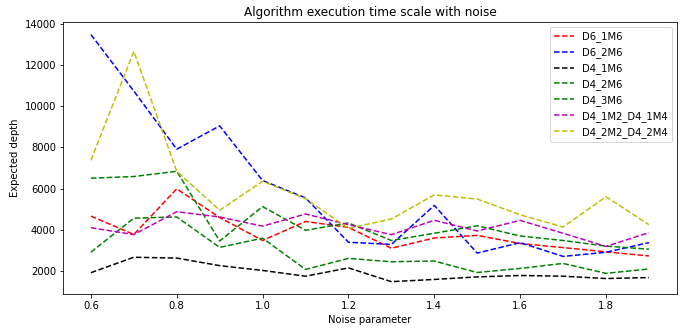
\includegraphics[width=13cm]{images/6_qubit_tests_.png}
\end{frame}

\begin{frame}{Tests on 6 qubits: results}
	\begin{itemize}
		\item Dm\_iM6 stands for algoritm with local Grover operator applied $i$ times
		\item We can see that some algorithms perform better than the others
		\item Some algorithms scale better with noise parameter. D6\_2M6 has lower expected depth than D4\_1M2\_D4\_1M4 at low noise parameter values, but greater at large noise parameter values
	\end{itemize}
\end{frame}

\begin{frame}{Задача 2: результаты измерений в таблице}
\centering
\begin{tabular}{lccc}
    Имя & Работа 1 & Работа 2 & Итог \\
\hline\hline
    Алиса & 8.0 & 9.0 & 8.5 \\
    Боб & 9.0 & 9.8 & 9.4 \\
    Чак & 9.1 & 9.3 & 9.2 \\
\end{tabular}

\begin{block}{Пояснения к таблице}
  \begin{itemize}
  \item Таблицы могут требовать пояснений.
  \item Что это за величины? Откуда они взялись?
  \item Какие выводы можно сделать?
  \end{itemize}
\end{block}

\end{frame}


\begin{frame}
\frametitle{Задача 2: результаты сравнения с конкурентами\footnote{Понятна ли ваша диаграмма? Не забыли ли вы легенду?}\footnote{Контрастно ли изображение? Помните, на проекторе всё может выглядеть хуже.}}
\begin{center}
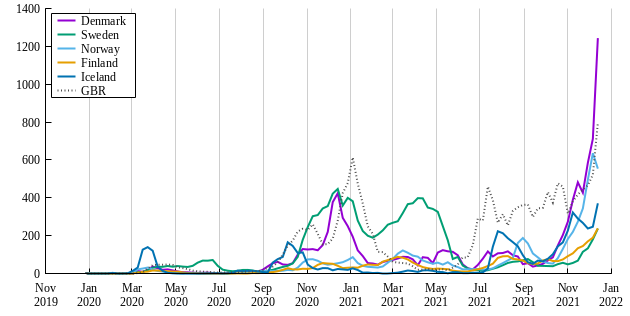
\includegraphics[width=11cm]{images/graph.png}
\end{center}
\end{frame}

\begin{frame}
\frametitle{Задача 3: основные трудности}
\begin{itemize}
\item Мы всё классно сделали, но рецензенты STOC сформулировали ряд претензий к~работе, обозвали нас идиотами и отказались пускать на конференцию.
\item Все замечания были исправлены, попробуем FOCS\footnote{Не забывайте про нежелательность англицизмов и аббревиатур.}!
\end{itemize}

\end{frame}

\begin{frame}
\frametitle{Дополнительный слайд по работе в целом\footnote{Кстати, слайды с длинными перечислениями выглядят плохо. Старайтесь их избегать.}}
\begin{itemize}
\item Освоенные и применённые технологии
\item Информация о внедрении
\item Полученные в ходе выполнения работы навыки
\item Вынесенные уроки
\item Реальные планы на будущее (не надо фантазировать!)
\item Ссылки на цитированную литературу --- их можно вынести в конец слайдов, но во время доклада не показывать.
\end{itemize}

\end{frame}


\begin{frame}
\frametitle{Результаты работы}

\begin{enumerate}
\item Разработан полиномиальный алгоритм решения задачи коммивояжёра.
\item Программная реализация демонстрирует высочайшую производительность и превосходит все известные аналоги.
\item Результаты подготовлены для представления на~FOCS.
\end{enumerate}

\vspace{5mm}\hrule\vspace{5mm}

\begin{center}
Имя, фамилия и контакты автора,\\ссылка на материалы работы, QR-код.
\end{center}

\end{frame}

\begin{frame}[noframenumbering,plain]
\frametitle{}
\begin{center}
  \Huge Спасибо за внимание!

  Ваши вопросы?

  {\color{red}Этот слайд не нужен! Удалите его\footnote{Сноски на слайдах тоже удалите: не нужно усложнять их структуру и содержимое. Не~забывайте, что многое можно просто сказать словами.}!}
\end{center}
\end{frame}



\end{document}
